\documentclass[conference]{IEEEtran}
\IEEEoverridecommandlockouts
% The preceding line is only needed to identify funding in the first footnote. If that is unneeded, please comment it out.
\usepackage{cite}
\usepackage{amsmath,amssymb,amsfonts}
\usepackage{algorithmic}
\usepackage{graphicx}
\usepackage{textcomp}
\usepackage{xcolor}
\usepackage{hyperref}
\usepackage{listings}
\usepackage{etoolbox}
\AtBeginEnvironment{quote}{\small}
\def\BibTeX{{\rm B\kern-.05em{\sc i\kern-.025em b}\kern-.08em
    T\kern-.1667em\lower.7ex\hbox{E}\kern-.125emX}}
% Expectation symbol
\DeclareMathOperator*{\E}{\mathbb{E}}
% Real number symbol
\DeclareMathOperator*{\R}{\mathbb{R}}
% Probability symbol
\DeclareMathOperator*{\Prob}{\mathbb{P}}
\DeclareMathOperator*{\N0}{\mathbb{N}_0}

\begin{document}

\title{Introduction to Stochastic Dynamic Programming}

\author{\IEEEauthorblockN{Chuan Tian Zhang}
\IEEEauthorblockA{\textit{Electrical and Computer Engineering} \\
\textit{University of Waterloo}\\
Waterloo, Ontario, Canada \\
ben.zhang@uwaterloo.ca}
}

\maketitle

\begin{abstract}
Dynamic programming is a popular technique to reduce the number of calculations required. This paper explores a variant of dynamic programming that deals with stochastic systems, where process noise is present. In this paper, stochastic optimal control problems are formulated using the Bellman equation and solved efficiently using dynamic programming. This paper is presented as a tutorial paper and focuses on the fundamentals of discrete-time stochastic control problems.
\end{abstract}

%\section{Introduction and Literature Review}
%
%TODO: introduce the reference papers, introduce the benchmark problem.

\section{Problem Formulation}

There are two well-known formulations of the discrete-time stochastic control problem. One formulation is in the state-space form and is analogous to its continuous-time equivalent. It lends itself well to solutions such as Linear Quadratic Gaussian (LQG) control. The other formulation uses state and action sets, and reward and state transition functions. A popular special case of this formulation is the Markov Decision Process (MDP). This formulation is often used when the intended solution is dynamic programming. Analysis of the equivalence of these two formulations is beyond the scope of this paper. We will outline both formulations below and use the latter in the rest of this paper.

\subsection{State-Space Formulation}

This section outlines the state-space formulation of a discrete-time stochastic control problem \cite{Rogers2010coursenotes,bertsekas1995dynamic}.

The state evolution of a discrete-time stochastic system is characterized by the following differential equation:
\begin{equation}
x_{k+1}=f_k(x_k,u_k,w_k)\label{stochastic_system}
\end{equation}
with initial condition $x_0 = x$. $k = 0,1,...,N$ represents the time step. When $N < \infty$ then the problem is finite-horizon. Otherwise it is infinite-horizon. $u_k$ is the control input at time $k$ and $w_k$ is the process noise at time $k$. $u_k$ is often a function of $\{x_0,x_1,...,x_k\}$. $w_k$ is drawn from some probability distribution. In theoretical analysis (e.g. LQG for linear systems) assumptions on the independence random variables (e.g. independent process noise, uncorrelated state and noise) are often present.
%We also make the following assumptions:
%\begin{enumerate}
%    \item Uncorrelated noise over time, i.e. $\E(w_i,w_j) = 0$ for all $i \neq j$
%    \item The initial condition is uncorrelated with noise.
%    \item TODO
%\end{enumerate}

The objective of optimal control is to find a control sequence $\{u^*_k\}$ where some cost function $J(\{x_k\},\{u_k\},\{w_k\})$ is minimized.

\subsection{Stochastic Dynamic Programming Formulation}

This section outlines the formulation of a discrete-time stochastic control problem useful for dynamic programming \cite{ross2014introduction}. We will use this formulation in subsequent sections.

The system is defined at each time step $k = 0,1,...,n$, where $n < \infty$ for a finite-horizon problem and $n = \infty$ for an infinite-horizon problem. The dynamics of the system is characterized by a set of feasible states $X_k$, a set of feasible actions $A_k$, and a state transition function $g_k: X_k \times A_k \rightarrow X_{k+1}$. Because this is a stochastic system, the transition function can be non-deterministic. For this reason, the probability density function of the transition function is defined to be $T_k: X_{k+1} \times X_k \times a_k \rightarrow \R = \Prob(x_{k+1}|x_k,a_k)$ where $T$ specifies the probability that taking action $a_k$ in state $X_k$ results in state $X_{k+1}$.

An immediate reward function $r_{k+1}: X_{k+1} \times A_k \rightarrow \R$ is also defined at each time step. The immediate reward function specifies the reward (a real number) for arriving at state $x_{k+1}$ after taking action $a_k$.
% Because $x_{k+1}$ can be non-deterministic in a stochastic system, we define the expected reward $\E(r_{k+1})$ as $\sum_{x_k \in X_k} \Prob()$

The objective of optimal control is to find a policy $\pi^*_k: X_k \rightarrow A_k$ such that following this policy (i.e. taking the action returned by $\pi^*_k$ at each time step $k$) maximizes the total reward $\sum_{k=1}^{n} r_k(x_k,a_{k-1})$. Because $x_k$ is the result of a stochastic process, the expected reward is defined as a part of the Bellman Equation in the next section.

\section{Bellman Equation}

In order to determine the optimal policy given a stochastic process (i.e. determine the best action to take at each $x_k$, where $x_{k+1}$ is drawn from a probability distribution), we define the expected reward $R_k$ for taking action $a_k$ in state $x_k$ as follows:
\begin{equation}
R_k(x_k,a_k)=\sum_{x_{k+1} \in X_{k+1}} \Prob(x_{k+1}|x_k,a_k) r_{k+1}(x_{k+1},a_k) \label{eq:immediate_expected_reward}
\end{equation}
Equation \eqref{eq:immediate_expected_reward} provides a way to find the maximum immediate reward $R^*_k$ for any given state:
\begin{equation}
R^*_k(x_k) = \max_{a_k \in A_k} R_k(x_k,a_k) \label{eq:max_immediate_expected_reward}
\end{equation}
The action that achieves the maximum immediate reward can also be found in \eqref{eq:max_immediate_expected_reward}.

Finding the action that achieves the best immediate reward is called the greedy algorithm. While efficient, the greedy algorithm is known to fail to provide the optimal policy over the entire horizon \cite{gutin2002traveling}. To fix this, Bellman introduced the concept of value functions as a way to quantify the total maximum expected reward in the entire horizon \cite{bellman1966dynamic}.

The value function is defined as follows:
\begin{equation}
\begin{aligned}
V_k(x_k) &= \max_{a_k \in A_k} \{ R_k(x_k,a_k) + \\
         & \gamma\sum_{x_{k+1} \in X_{k+1}} \Prob(x_{k+1}|x_k,a_k) V_{k+1}(x_{k+1}) \}, \\
V_n(x_n) &= 0,\\
k &= 1,2,...,n,\\
\gamma &\in [0, 1]
\label{eq:value_function}
\end{aligned}
\end{equation}
Equation \eqref{eq:value_function} denotes that at time step $k$, the value of state $x_k$ is the maximum expected immediate reward plus the expected value of future states (after taking action $a_k$) multiplied by discount factor $\gamma$. $\gamma$ is a way of specifying the preference of near-term rewards over long-term rewards. It also helps keep the value finite in infinite-horizon problems. This is called the Bellman Equation.

The optimal policy is then the $a_k$ that achieves the value $V_k(x_k)$ (maximizes the expression in \eqref{eq:value_function}). This result follows from the proof of Bellman's principle of optimality, which states that ``An optimal policy has the property that whatever the initial state and initial decision are, the remaining decisions must constitute an optimal policy with regard to the state resulting from the first decision'' \cite{bellman1966dynamic}.

To gain an intuitive sense of the value function, consider the last time step where we can take action (i.e. $k=n-1$).
\begin{equation}
\begin{aligned}
V_{n-1}(x_{n-1}) &= \max_{a_{n-1} \in A_{n-1}} \{ R_{n-1}(x_{n-1},a_{n-1}) + \\
         & \gamma\sum_{x_n \in X_n} \Prob(x_n|x_{n-1},a_{n-1}) V_n(x_n) \} \\
         &= \max_{a_{n-1} \in A_{n-1}} \{ R_{n-1}(x_{n-1},a_{n-1})\}
\label{eq:value_function_example}
\end{aligned}
\end{equation}
This is the same as the greedy algorithm, where we choose the action that yields the best expected reward. This gives us the optimal policy for $k=n-1$:
\begin{equation}
\pi^*_{n-1}(x_{n-1}) = arg\max_{a_{n-1} \in A_{n-1}} \{ R_k(x_{n-1},a_{n-1})\}
\label{eq:value_function_example_optimal_policy}
\end{equation}

Assuming that we act according to the optimal policy from time step $i < n$, by Bellman's principle of optimality, the value function gives us the optimal policy for time step $i - 1$. By induction, we then have the optimal policy for each time step.

\section{Solution Methods for the Bellman Equation}

\subsection{Finite-Horizon}

The Bellman equation is a recursive function, where $V_{k}$ depends on $V_{k+1}$,  $k=0,1,...,n-1$. Since the expected reward functions $R_k$ and transition probabilities $\Prob(x_{k+1}|x_k,a_k)$ are given in the problem formulation, we can employ the standard methods for efficiently solving recursive functions such as memoization. Alternatively, we can work backwards from time step $n$ and obtain $V_k(x_k)$ for all $k = 0,1,...,n$ and $x_k \in X_k$.

\subsection{Infinite-Horizon}

Assuming that $R_k$ grows slower than $\gamma^k$ decays with respect to $k$, the value function is finite. We can then use the same recursive with memoization method as the finite-horizon case, except we stop when the value function converges instead of reaching time step $n$.

\subsection{Stationary value function}

One variant of the dynamic programming problem presented above uses a stationary value function on time-invariant state and action spaces. i.e. \eqref{eq:value_function} becomes:
\begin{equation}
\begin{aligned}
V(x) &= \max_{a \in A} \{ R(x,a) + \\
         & \gamma\sum_{x' \in X} \Prob(x'|x,a) V(x') \}
\label{eq:stationary_value_function}
\end{aligned}
\end{equation}
This results in the widely studied Markov Decision Process (MDP) \cite{bellman1957markovian}. Some solution methods for MDP are value iteration \cite{bellman1957markovian}, policy iteration \cite{howard1960dynamic}, and approximation methods for improving the computational efficiency of the solution \cite{van1976set,puterman1978modified}.

\section{Example Problem}

To experimentally observe the performance of stochastic dynamic programming, we will analyze a classic gambler's ruin problem as proposed in \cite{winston2004operations}. The original problem is quoted below:
\begin{quote}
A gambler has \$2. She is allowed to play a game of chance four times, and her goal is to maximize her probability of ending up with a least \$6. If the gambler bets $b$ dollars on a play of the game, then with probability $0.4$, she wins the game and increases her capital position by $b$ dollars; with probability $0.6$, she loses the game and decreases her capital by $b$ dollars. On any play of the game, the gambler may not bet more money than she has available. Determine a betting strategy that will maximize the gambler’s probability of attaining a wealth of at least \$6 by the end of the fourth game. We assume that bets of zero dollars (that is, not betting) are permissible.
% Alternative problem:
% Given a set of vertices $X$, each with two edges $A$ and $B$. Each edge has an associated cost. A robot is tasked with finding the optimal path starting from $x_s \in X$ and ending in $x_f \in X$. The robot's actuators are faulty and if the robot chooses to go along edge $A$, it has a probability $p$ of going along edge $A$ and probability $1-p$ of going along edge $B$. Find an optimal policy for the robot to go from state $x_s$ to $x_f$.
\end{quote}
For the purpose of our analysis, assume that the plays are pairwise independent (similar to a perfect dice roll, where each roll is independent of any other roll).

Notice that because of the independence assumption, betting $b$ dollars per round for 2 rounds yield identical returns to betting $2b$ dollars in one round. This is shown below:
\begin{equation}
\begin{aligned}
\E(r_a) &= pb+pb = 2pb\\
\E(r_b) &= p(2b) = 2pb = \E(r_a)
\end{aligned}
\end{equation}
where $r_a$ is the return after betting $b$ dollars per round for 2 rounds, $r_b$ is the return after betting $2b$ dollars for one round, and $p$ is the probability of winning ($0.4$ in the original problem).

Therefore, a strategy to maximize the chance that the gambler ends up with at least $G$ dollars is to place a bet of $max(0,min(x, G-x))$ dollars in each round, where $x$ is the current wealth. Intuitively, this means that we place the maximum amount of bet per round needed to close the gap between the current wealth $x$ and the target wealth $G$. We will call this the greedy algorithm.

The same problem can be formulated as a discrete-time finite-horizon stochastic dynamic programming problem.
The state-space is the space of non-negative integers: $X = \N0$.
The action space is the bet amount $b \ge 0$, where $b_k \le x_k$ in each time step $k$.
The transition probability is characterized by:
\[ x_{k+1} =
\begin{cases} 
  x_k + b & \text{with probability } 0.4 \\
  x_k - b & \text{with probability } 0.6 \\
\end{cases}
\]
The immediate reward is $1$ when the new wealth is \$6 or above and $0$ otherwise. Because this is a finite-horizon problem and the result is a binary win/lose, set the discount factor $\gamma$ to weigh all rewards equally. Note that this formulation gives us the theoretical winning probability in the value function $V_0(x_0)$.

\subsection{Convergence to Theoretical Winning Probability}

\begin{figure}[htbp]
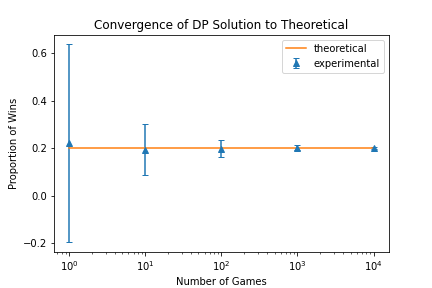
\includegraphics[width=\columnwidth]{dp-convergence.png}
\caption{Graph showing the convergence of the experimental dynamic programming winning probability to the theoretical dynamic programming winning probability. The blue triangle is the mean and the blue lines denote the standard deviation. The experiment is carried out with the original problem formulation.}
\label{dp-convergence}
\end{figure}

To gain confidence that the value function gives us the theoretical winning probability, We can experimentally show that the experimental proportion of wins is close to theoretical. In Fig.~\ref{dp-convergence} we see that as we play more games, the sample mean and sample standard deviation of the proportion of wins converge to the theoretical winning probability. In subsequent experiments (excluding performance benchmarks), we will compare the experimental result from the greedy algorithm with the theoretical results from the dynamic programming formulation, in order to reduce computational burden and noise. We will use $100000$ as the number of games in subsequent experiments unless stated otherwise.

\subsection{Performance Comparison (Proportion of Wins)}

In this section, we will benchmark the stochastic dynamic programming algorithm alongside the greedy algorithm in terms of the proportion of wins. We will vary parameters of the original problem and graph the performance (proportion of wins) of each algorithm for comparison.

\begin{figure}[htbp]
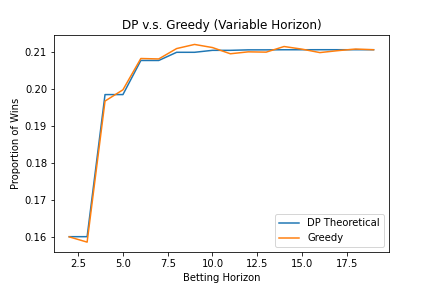
\includegraphics[width=\columnwidth]{dp-vs-greedy-variable-horizon.png}
\caption{Graph showing the theoretical performance of the dynamic programming algorithm compared with the experimental performance of the greedy algorithm. All parameters except for the variable betting horizon are consistent with the original problem formulation.}
\label{dp-vs-greedy-variable-horizon}
\end{figure}

\begin{figure}[htbp]
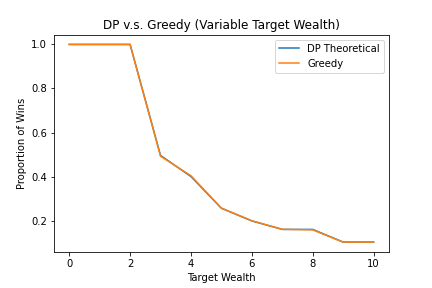
\includegraphics[width=\columnwidth]{dp-vs-greedy-variable-target-wealth.png}
\caption{Graph showing the theoretical performance of the dynamic programming algorithm compared with the experimental performance of the greedy algorithm. All parameters except for the variable target wealth are consistent with the original problem formulation.}
\label{dp-vs-greedy-variable-target-wealth}
\end{figure}

\begin{figure}[htbp]
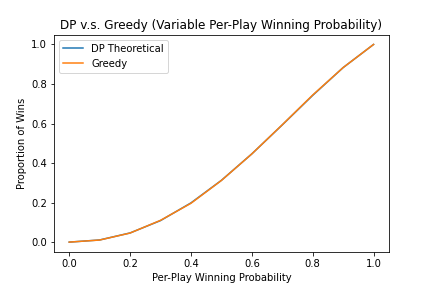
\includegraphics[width=\columnwidth]{dp-vs-greedy-variable-per-play-winning-prob.png}
\caption{Graph showing the theoretical performance of the dynamic programming algorithm compared with the experimental performance of the greedy algorithm. All parameters except for the variable per-play winning probability are consistent with the original problem formulation.}
\label{dp-vs-greedy-variable-per-play-winning-prob}
\end{figure}

\begin{figure}[htbp]
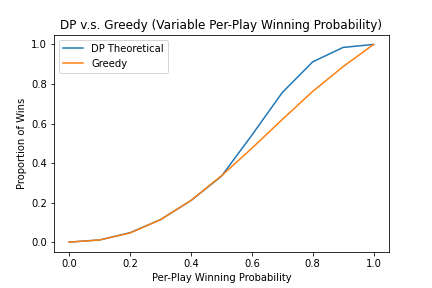
\includegraphics[width=\columnwidth]{dp-vs-greedy-variable-per-play-winning-prob-and-betting-horizon-10.png}
\caption{Graph showing the theoretical performance of the dynamic programming algorithm compared with the experimental performance of the greedy algorithm. All parameters except for the betting horizon (set to 10) and the variable per-play winning probability are consistent with the original problem formulation.}
\label{dp-vs-greedy-variable-per-play-winning-prob-and-betting-horizon-10}
\end{figure}

\begin{figure}[htbp]
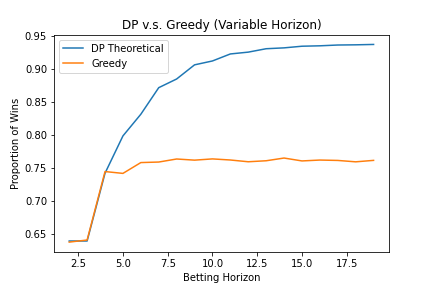
\includegraphics[width=\columnwidth]{dp-vs-greedy-variable-horizon-and-per-play-winning-prob-0_8.png}
\caption{Graph showing the theoretical performance of the dynamic programming algorithm compared with the experimental performance of the greedy algorithm. All parameters except for the per-play winning probability (set to $0.8$) and  the variable betting horizon are consistent with the original problem formulation.}
\label{dp-vs-greedy-variable-horizon-and-per-play-winning-prob-0_8}
\end{figure}

Figs.~\ref{dp-vs-greedy-variable-horizon},~\ref{dp-vs-greedy-variable-target-wealth},~\ref{dp-vs-greedy-variable-per-play-winning-prob} show that there is no significant performance differences between the dynamic programming solution and the greedy solution when individually varying the betting horizon, target wealth, or per-play winning probability. However, as shown in Figs.~\ref{dp-vs-greedy-variable-per-play-winning-prob-and-betting-horizon-10}~and~\ref{dp-vs-greedy-variable-horizon-and-per-play-winning-prob-0_8}, when the per-play winning probability is high ($> 0.5$) and the betting horizon is high ($> 4$), the dynamic programming algorithm vastly outperforms the greedy approach. This may be because:
\begin{enumerate}
    \item when the betting horizon is small, the greedy algorithm's lack of look-ahead does not impact the performance significantly.
    \item when the per-play winning probability is low, the riskiness of the optimal move is high, which happens to make the dynamic programming algorithm take the same ``all-or-nothing'' approach as the greedy algorithm.
\end{enumerate}

\subsection{Performance Comparison (Computational Performance)}

\begin{figure}[htbp]
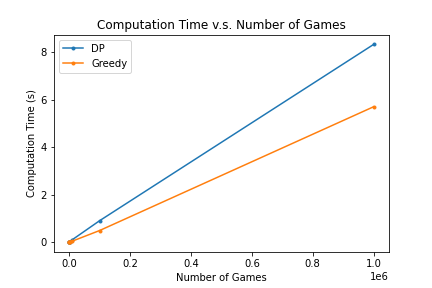
\includegraphics[width=\columnwidth]{dp-vs-greedy-computation-time.png}
\caption{Graph showing the computational performance of the dynamic programming algorithm and the greedy algorithm with changing number of games.}
\label{dp-vs-greedy-computation-time}
\end{figure}

\begin{figure}[htbp]
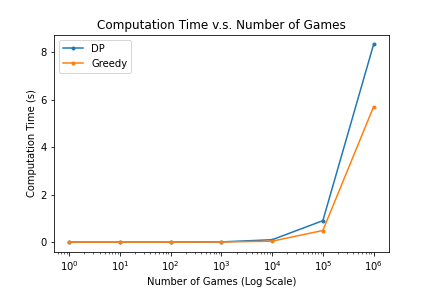
\includegraphics[width=\columnwidth]{dp-vs-greedy-computation-time-log.png}
\caption{Graph showing the computational performance of the dynamic programming algorithm and the greedy algorithm with changing number of games. The x axis is a log scale.}
\label{dp-vs-greedy-computation-time-log}
\end{figure}

\begin{figure}[htbp]
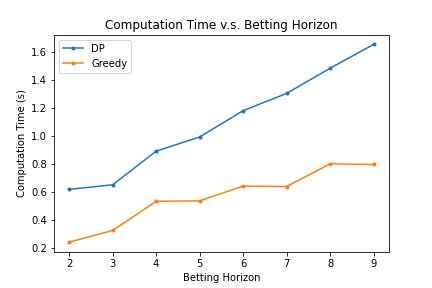
\includegraphics[width=\columnwidth]{dp-vs-greedy-computation-time-vs-betting-horizon.png}
\caption{Graph showing the computational performance of the dynamic programming algorithm and the greedy algorithm with changing betting horizon.}
\label{dp-vs-greedy-computation-time-vs-betting-horizon}
\end{figure}

In this section, we will benchmark the stochastic dynamic programming algorithm alongside the greedy algorithm in terms of computational performance.

Figs.~\ref{dp-vs-greedy-computation-time},~\ref{dp-vs-greedy-computation-time-log} show that both the dynamic programming algorithm and the greedy algorithm scale linearly with the number of games, and the scaling term is smaller for the greedy algorithm and larger for the dynamic programming problem. Fig.~\ref{dp-vs-greedy-computation-time-vs-betting-horizon} shows that the computation time for both algorithms is also linear to the betting horizon.

\subsection{Experimental Takeaways}

By the formulation of the stochastic dynamic programming solution, we can ensure that our solution is optimal in terms of maximizing the expected probability of reaching the goal. However, for small problems, the greedy algorithm performs just as well with less computation power.

The experimental results can be reproduced with the code found in \cite{zhang2021}.

\section{Limitations}

Stochastic dynamic programming has a major drawback known as the curse of dimensionality \cite{Rogers2010coursenotes}. When solving the Bellman equation as described in \eqref{eq:value_function}, the value function lookup table grows quickly with respect to the planning horizon. Suppose the size of each state space $X_k$ is $N_X$, the size of each action space $A_k$ is $N_A$, and the number of time steps is $n$. Then the total number of function evaluations is $N_XN_An$. For moderately large state space, action space, or planning horizon, the space and computational requirements become paramount. To solve this issue, various approximation approaches have been proposed \cite{powell2007approximate}.

\section{Conclusions}

This tutorial paper explored the field of stochastic dynamic programming, including the problem formulation, deriving the Bellman equation for solving for an optimal policy, outlining the solution methods to the Bellman equation, and benchmarking the stochastic dynamic programming approach with a baseline greedy approach. While the greedy approach is computationally efficient and doesn't require much space, the dynamic programming approach yields the optimal solution.

% Bibliography

% The following statement selects the style to use for references.  
% It controls the sort order of the entries in the bibliography and also the formatting for the in-text labels.
\bibliographystyle{plain}
% This specifies the location of the file containing the bibliographic information.  
% It assumes you're using BibTeX to manage your references (if not, why not?).
\cleardoublepage % This is needed if the "book" document class is used, to place the anchor in the correct page, because the bibliography will start on its own page.
% Use \clearpage instead if the document class uses the "oneside" argument
\bibliography{references}
% Tip: You can create multiple .bib files to organize your references. 
% Just list them all in the \bibliogaphy command, separated by commas (no spaces).

\end{document}
